\section{Results}
\label{sec-results}
%\input graphsize_table

We will analyse search performance as follows: 
First, we look at the effectiveness of our new online and offline symmetry
reduction methods using results published in \cite{harabor10} as a 
comparative baseline.
Next, we compare and contrast the performance of our new algorithm with that
of another similar method recently described in the literature \cite{pochter10}.
Finally, we demonstrate the relative strengths and weaknesses of these two
techniques by scaling all maps in our benchmark sets by a factor of 3 and looking
at the effect this has on performance.


\begin{figure*}[t]
       \begin{center}
                       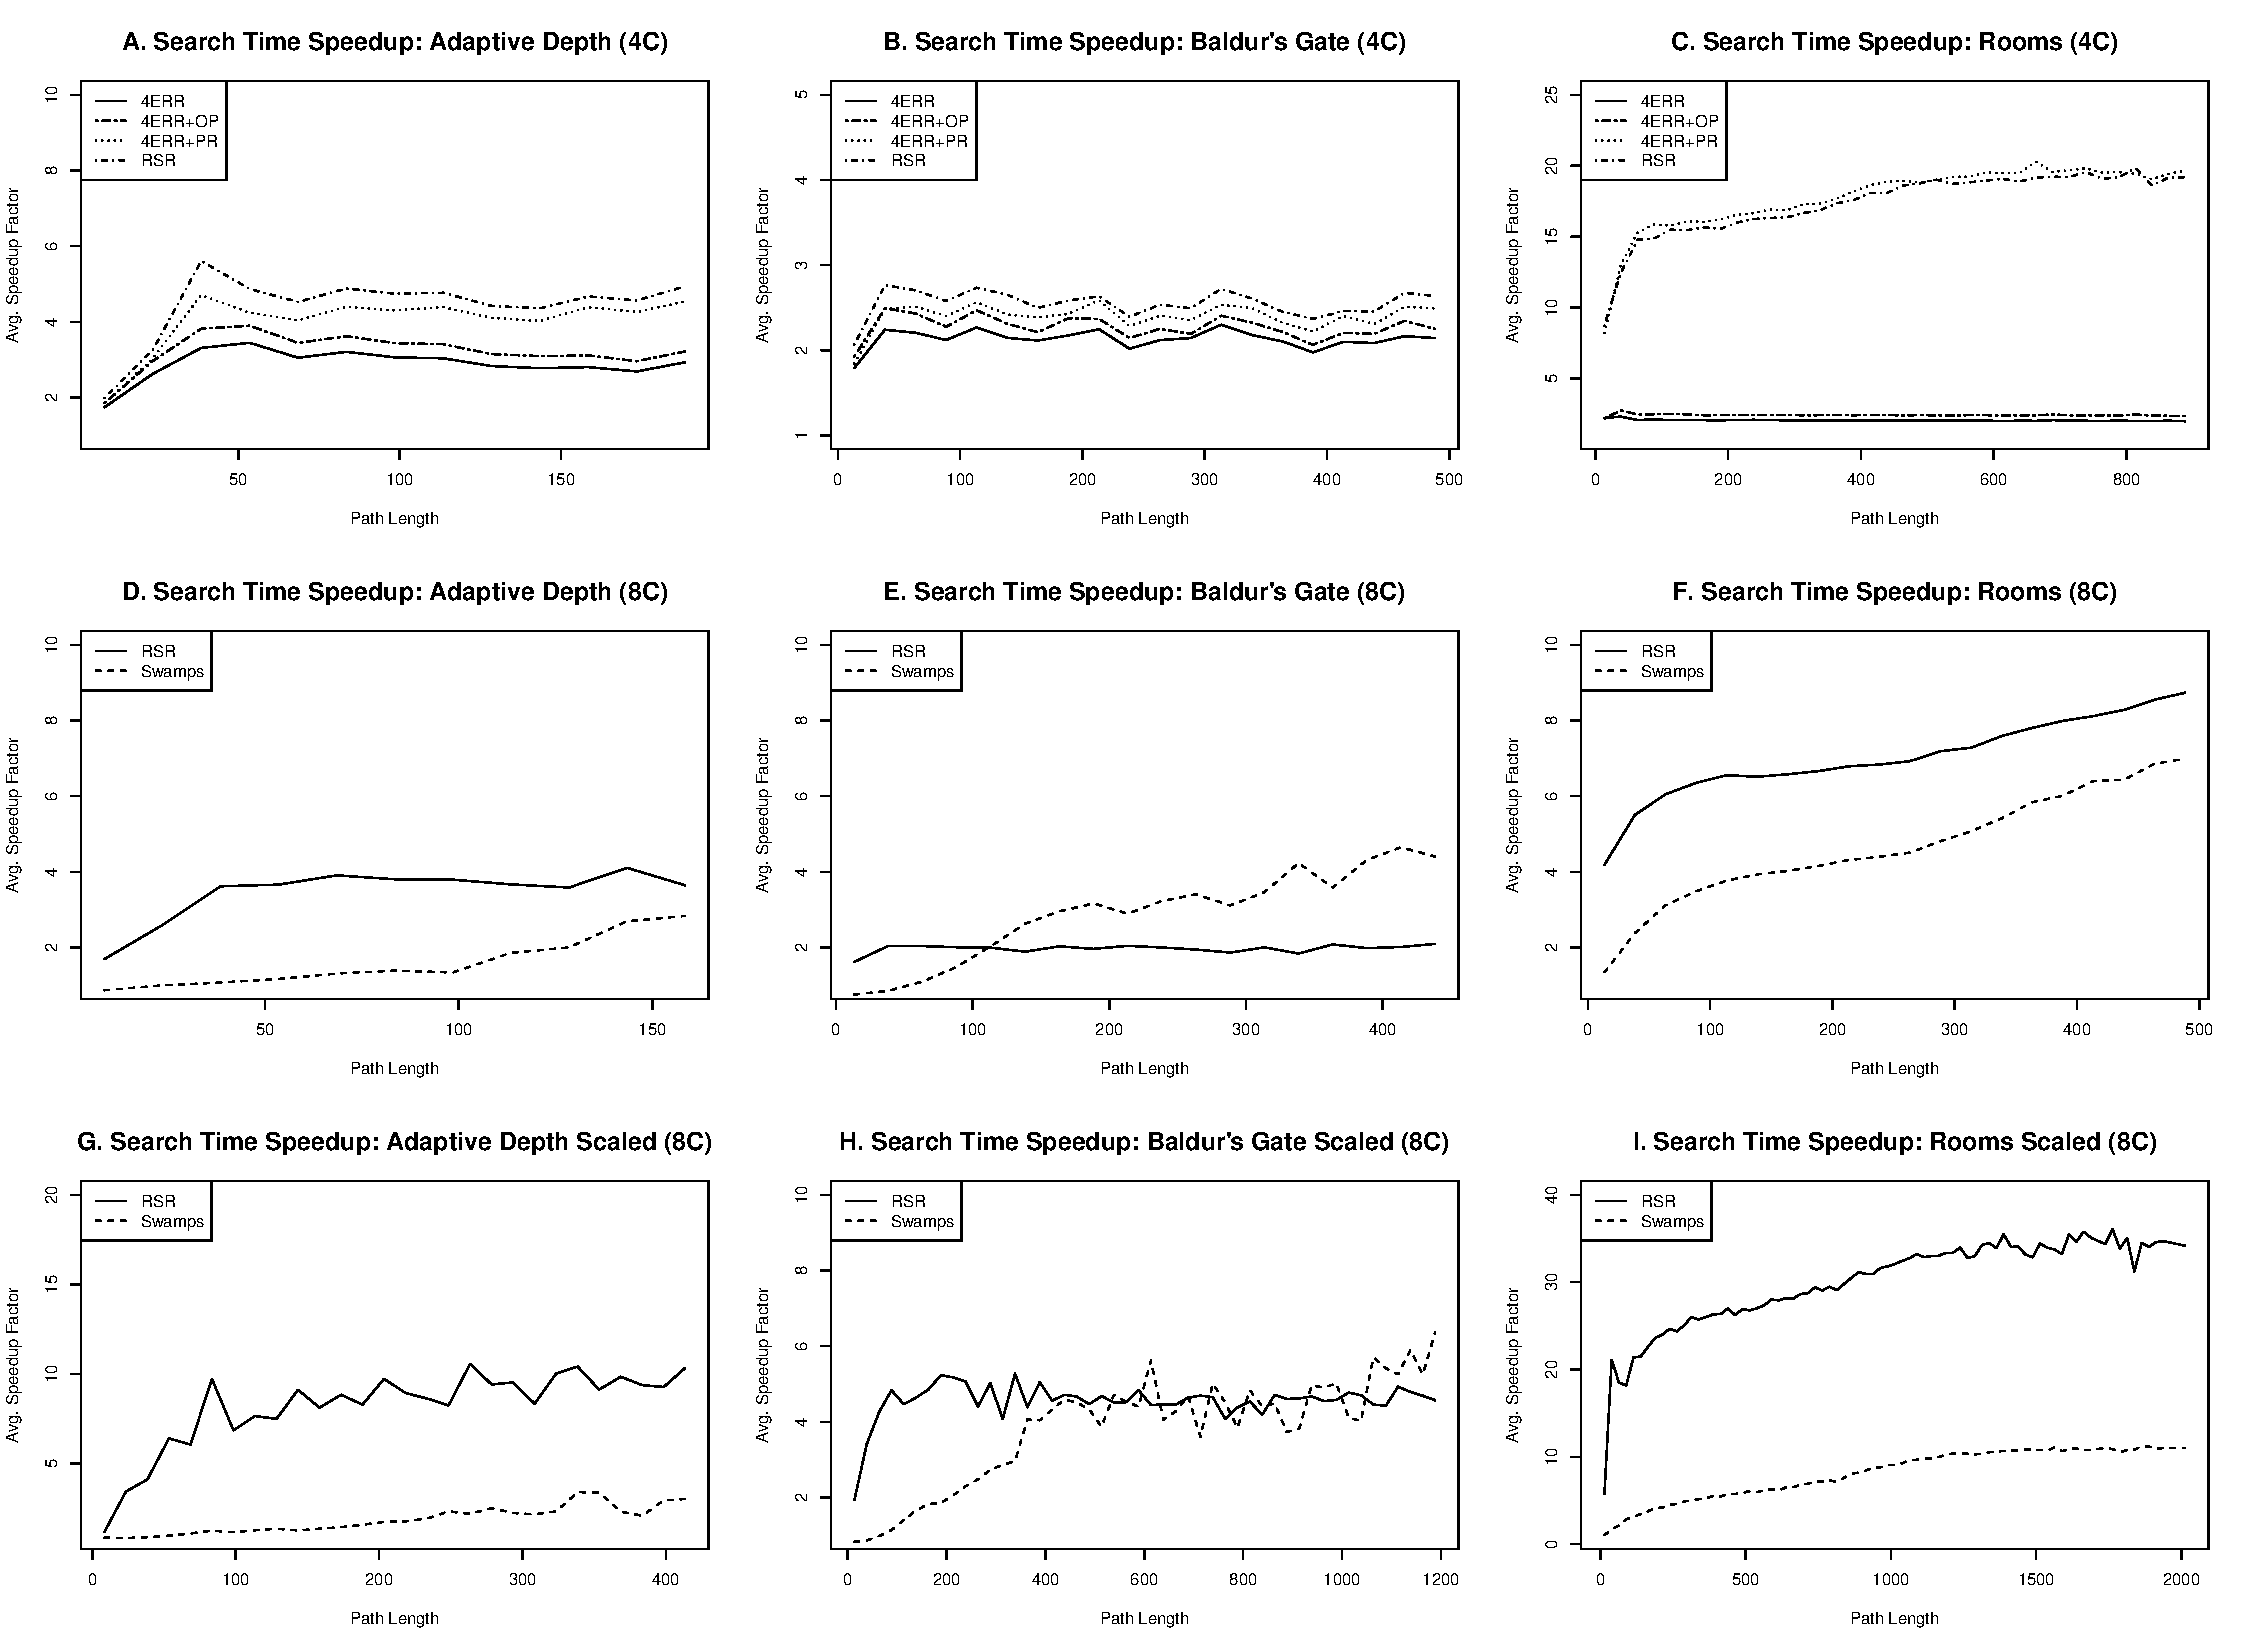
\includegraphics[width=1.95\columnwidth, trim = 10mm 10mm 10mm 0mm]{diagrams/speedup.pdf}
       \end{center}
       \caption{Average A* speedup on each of our three benchmarks. 
		Results are given in terms of nodes expanded and search time.}
\label{fig-speedup}
\end{figure*}

\textbf{Symmetry Reduction Improvements: }
In Figure \ref{fig-speedup} (A to C) we report on the  
effectiveness of offline perimeter reduction (PR) and on-the-fly 
node pruning (OP) to speeding up A* search on 4-connected grid maps.
Our baseline comparison is the Rectangular Room Symmetry Reduction algorithm 
(RRSR) originally described in \cite{harabor10}.
\par
Perhaps the first thing to note is that the single biggest improvement on each
benchmark is observed when applying perimeter reduction to the basic RRSR method.
In the case of the Rooms benchmark (Figure \ref{fig-speedup}C) RRSR+PR is over 9
times faster than RRSR alone and up to 19 times faster than A* search on an unmodified
grid map.
Smaller but still significant gains are also observed on the remaining two benchmarks:
on Adaptive Depth (Figure \ref{fig-speedup}A) RRSR+PR is twice as fast as RRSR alone
and performance on Baldur's Gate (Figure \ref{fig-speedup}B) is improved by over 10\%.
By comparison, on-the-fly node pruning yields much smaller gains across the same benchmarks:
both RRSR+OP and RRSR+PR+OP only improve the search performance by 10\% on the majority
of problem instances.
\par
Finally, it is interesting to note the sometimes large performance variation 
from one benchmark to another. This is indicative of how effectively we can 
decompose the different maps into rectangular shaped regions.
For example, the maps in the Rooms set are highly suited to this approach but those
from Baldur's Gate, which have an unusual 45-degree orientation, are not.
In such cases there are fewer opportunities to apply perimeter reduction and this 
leads to larger search spaces and reduced performance. 
\par
\textbf{Comparative Anaysis vs. Swamps Reduction:}
Next, we compare the speedup performance of RSRR+PR+OP with the Swamps algorithm 
described in \cite{pochter10}. Swamps is an alternative search space reduction 
which requires decomposing a graph into so called ``swamp'' areas that can be 
ignored because a there always exists a symmetric path that does not cross any 
tiles in the swamp. 
Each search instance is then limited to an a corridor of inter-dependent 
swamps (and non-swamp areas) and all remaining nodes in the graph are ignored.
To evaluate Swamps we used the author's source code from \cite{pochter10} and
ran all experiments using their recommended running parameters\footnote{To the best of our knowledge 
these parameters are unpublished; they were recommended to us in a private communique.}:
 a Swamp seed radius of 6 and ``no change limit'' of 2.
\par
Figure \ref{fig-speedup} (D to F) gives search time speedup results for both 
RRSR+PR+OP and Swamps running on the 8-connected variants of our three benchmark 
problem sets. 
On Adaptive Depth (Figure \ref{fig-speedup}E), we observe that 
Swamps yields a maximum search time speedup of 2.8 times faster than 
 A* running on an unmodified grid map; however this is only true for problems of length greater than 150.
By comparison RSRR+PR+OP yields a maximum speedup of 4.1 with comparatively little fluctuation across the
large majority of probem instances.
On Baldur's Gate (Figure \ref{fig-speedup}E) this trend is almost reversed; RRSR+PR+OP consistently 
yields search time speedups of factor 2 while Swamps exhibits a maximum speedup of 4.4.
Finally, on Rooms (Figure \ref{fig-speedup}F) RSRR+PR+OP is again shown to be faster than Swamps;
usually by a factor of between 2 and 3 across most problem instances.
\par
It is interesting to observe that on the benchmarks which RRSR+PR+OP does best (Rooms, Adaptive Depth) 
there are usually large open areas and the terrain can be naturally decomposed into rectangular areas. 
At the same time, Swamps-based reduction appears to be much better suited for identifying symmetric paths 
in graphs where this is not the case.
It seesms reasonable then to try and answer whether this trend is true more generally.
To accomplish this we scaled up each map in every benchmark by a factor of 3 and randomly generated a new
set of 100 problem instances per map and observe the effect this has on average speedup for problems of the 
same length as those generated on the un-scaled maps.




